\documentclass{report}

\usepackage[T1]{fontenc}
\usepackage[utf8]{inputenc}
\usepackage[francais]{babel}
\usepackage{graphicx}
\usepackage{mathptmx}
\usepackage{fancyhdr}
\usepackage[headheight=110pt,a4paper,margin=2.5cm]{geometry}
\usepackage{setspace}
\usepackage[chapter]{algorithm}
\usepackage{subcaption}
\usepackage{titletoc}
\usepackage{amsmath}
\usepackage{amssymb}
\usepackage{enumitem}
\usepackage{adjustbox}
\usepackage{multirow}
\usepackage{array}
\usepackage{textcomp}
\usepackage{gensymb}
\usepackage{apacite}
\usepackage{booktabs}
\usepackage{chngcntr}
\usepackage{emptypage}
\usepackage{nameref}


\renewcommand\thesection{\arabic{section}.}


\begin{document}

    \begin{titlepage}
  \begin{center}

    % Logo
    \includegraphics[scale=0.5]{images/logo_paris_sud}~\\[0.5cm]

    \textsc{\LARGE Université Paris-Sud}\\[1.25cm]
    
    \textsc{\LARGE Master AIC}\\[0.5cm]

    \textsc{\Large TC5 - Traitement des Images et du Signal}\\[1.5cm]
    
    \textsc{\LARGE Rapport de projet}\\[0.5cm]

    % Title
    \rule{\linewidth}{0.5mm} \\[0.4cm]
    { \huge \bfseries Reconnaissance faciale en utilisant les eigenfaces\\[0.4cm] }
    \rule{\linewidth}{0.5mm} \\[2cm]

    % Author(s)
    \begin{minipage}{0.9\textwidth}
      \begin{flushleft} \LARGE
        Auteurs :\\
        Ghiles \textsc{Sidi Said}\\
        Mohamed Ali \textsc{Darghouth}\\
        Walid \textsc{Belrhalmia}\\
      \end{flushleft}
    \end{minipage}

    \vfill

    % Bottom of the page
    {\LARGE{\today}}

  \end{center}
\end{titlepage}
    \newpage
    
    \tableofcontents
    \newpage
    
    \listoffigures
    \newpage
    
    
    \chapter*{Introduction}
    \addcontentsline{toc}{chapter}{Introduction}
    La reconnaissance faciale est une méthode de reconnaissance biométrique
qui consiste en l'identification d'un individu à partir d'une image de son
visage. Étant donné qu'un visage est unique à une personne (sauf dans des cas très
rares de jumeaux identiques où même un être humain ne peut pas faire 
la différence), la reconnaissance faciale est très adaptée pour l'identification
d'un individu.

La reconnaissance faciale a fait l'objet de plusieurs travaux de recherche ces dernières décennies,
on la retrouve aujourd'hui dans plusieurs secteurs de la vie quotidienne comme les systèmes de
contrôle d'accès, les systèmes de registre de présence, mais également dans les réseaux sociaux.

Dans ce projet, nous avons travaillé sur l'article \cite{} qui propose une méthode
basée sur les vecteurs propres des images de visages (appelés ``eigenfaces'', ce qui pourrait être 
traduit en ``visages propres'' en français. Par la suite nous allons utiliser le terme ``eigenfaces'').
C'est une méthode peu coûteuse en puissance de calcul, ce qui contraste avec les méthodes standards
actuelles qui utilisent des modèles obtenus par apprentissage profond (Deep Learning) qui nécessitent un
temps et une puissance de calcul considérables pour être appris, mais dont le taux de réussite aujourd'hui
atteint les 99\%.

Dans ce rapport, nous allons dans un premier temps expliquer la méthode proposée par \cite{} et
montrer les résultats obtenus. Ensuite, nous allons présenter notre propre implémentation de la méthode
ainsi que les résultats que nous avons obtenu. Enfin, nous allons étudier la robustesse de la méthode
aux bruits, à l'inversion de contraste, à la rotation, et à la translation.
    
    \chapter{Méthode proposée par l'article et résultats obtenus}
    Dans ce chapitre, nous allons d'abord présenter ce qu'on appelle les ``eigenfaces''.
Nous allons ensuite faire une brève présentation de la méthode de classification
``bayésien naïf''. Nous exposerons alors les différentes étapes de la méthode proposé
par \cite{article} ainsi que les résultats obtenus. Nous finirons par une critique de
la démarche de test de \cite{article}.


\subsection{Présentation des eigenfaces} \label{subsection:presentation_eigenfaces}
Soit un ensemble d'images de visages. On transforme chaque image, qui est un signal
discret à deux dimensions, en un vecteur à une dimension (on travaille avec des
images en niveaux de gris). On calcule alors la matrice de variance-covariance
de ces vecteur. On appelle eigenfaces les vecteurs propres de cette matrice.

Plus formellement : soit l'ensemble d'images $\{I_1, I_2, ..., I_M\}$.
Les étapes pour trouver les eigenfaces sont :
\begin{enumerate}
    \item Transformer chaque image $I_i$, qui est en deux dimensions,
    en un vecteur $\Gamma_i$ à une dimension.
    \item Calculer le vecteur moyen $Y$ : $Y = \frac{1}{M} \sum_{i=1}^M \Gamma_i$.
    \item Soustraire le vecteur moyen $Y$ de chaque vecteur $\Gamma_i$ : $\phi_i = \Gamma_i - Y$.
    \item Calculer $C$, la matrice variance-covariance des vecteurs $(\phi_i)_{i=1}^M$ :
    $C = A^TA$, où la ligne $i$ de $A$ est $\phi_i$.
    \item Calculer la matrice $u$, dont chaque colonne correspond à un vecteur
    propre de $C$. Les colonnes de $u$ sont les eigenfaces.
\end{enumerate}
Si $N$ est le nombre de pixels d'une image, alors $C$ est une matrice $N \times N$.
Pour $N$ assez grand (ce qui est très souvent le cas quand on travaille sur des images),
le calcul des vecteurs propres de $C$ devient vite très coûteux. Au lieu de faire cela,
on calcule les vecteurs propres de $AA^T$ (ils sont au nombre de $M$, le nombre d'images,
sachant que dans la plupart des cas $M << N$). Alors, pour chaque vecteur propre $v$ de
$AA^T$, $u = Av$ est un vecteur propre de $C$. Ça nous permet d'obtenir $M$ vecteurs
propres ($M$ étant le nombre d'images) qui sont considérés les eigenfaces et qui forment
une base de l'espace vectoriel des images.


\subsection{Classification bayésienne}
Soit un problème de classification où les individus sont représentés
par la variable aléatoire $X$ et les classes par la variable aléatoire $Y$.
La classification bayésienne repose sur le fait de classer un individu $x$ dans la
classe $y$ qui maximise la probabilité : $P(Y=y|X=x)$.

Le théorème de Bayes nous dit que :
\[
    P(Y=y|X=x) = \frac{P(X=x|Y=y) \times P(Y=y)}{P(X=x)}
\]
Donc pour maximiser $P(Y=y|X=x)$, il suffit de maximiser $P(X=x|Y=y) \times P(Y=y)$
(puisque $P(X=x)$ ne dépend pas de $y$ et nous cherchons à maximiser selon $y$).
On peut facilement estimer $P(Y=y)$ (par un simple comptage dans l'échantillon par exemple).
Le problème réside dans le calcul de $P(X=x|Y=y)$ sachant que $X$ est dans $\mathbb{R}^d$, 
c.a.d. que $X = (X_1, X_2, ..., X_d)$ où $X_i \in \mathbb{R}$.

L'hypothèse ``naïve'' sur laquelle se base la classification bayésienne est de supposer
les variables aléatoires $X_i$ indépendantes (d'où le nom ``bayésien naïf'' ou ``naïve bayes''
en anglais). Quand on fait cette hypothèse, il devient plus facile de calculer $P(X=x|Y=y)$.
En effet :
\[
    P(X=x|Y=y) = P(X_1=x_1, X_2=x_2, ..., X_d=x_d|Y=y) = \prod_{i=1}^d P(X_i=x_i|Y=y)
\]
Il suffit alors d'estimer $P(X_i|Y=y)$ pour chaque $i \in \{1, 2, ..., d\}$, ce qui est bien
plus facile à faire, et requière beaucoup moins de paramètres à estimer que dans le cas où
on devrait estimer $P(X|Y=y)$. Les hypothèses les plus couramment utilisées sur $P(X_i|Y=y)$
sont que la distribution est gaussienne ou binomiale.


\subsection{Étapes de la méthode}
Comme le montre la figure \ref{fig:article:etapes}, la méthode de décompose en deux 
étapes : apprentissage du modèle et déploiement du modèle.
\begin{figure}[H]
    \centering
    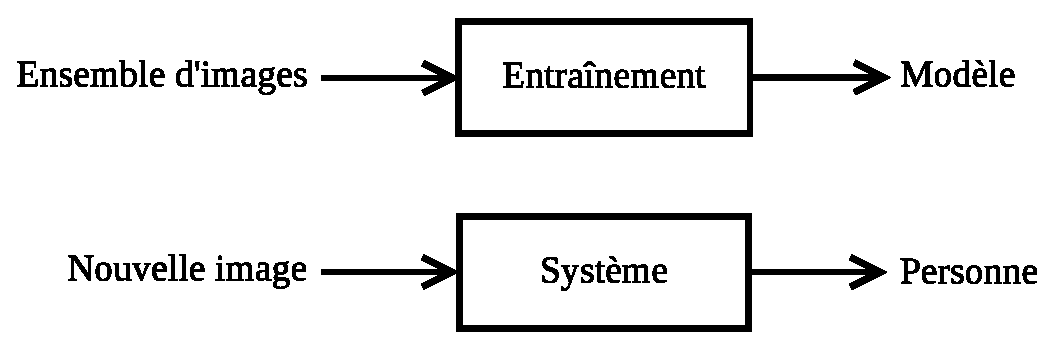
\includegraphics[scale=0.5]{images/article_etapes}
    \caption{Étapes de la méthode de \cite{article}.}
    \label{fig:article:etapes}
\end{figure}
Toutes les images sont préalablement converties en niveaux de gris.

\subsubsection{Apprentissage du modèle}
On utilise un classifieur bayésien dans lequel on suppose que $P(X_i|Y=y)$ suit une distribution
gaussienne ($X_i|Y=y \sim N(\mu_{iy}, \sigma_{iy})$).
L'étape d'apprentissage permet d'estimer les paramètres du modèle ($\mu_{iy} et
\sigma_{iy}$ pour chaque i et chaque y).
La figure \ref{fig:article:etapes_apprentissage} montre les différentes étapes
de l'apprentissage, celles-ci sont :
\begin{enumerate}
    \item À partir des images d’entraînement, calculer les eigenfaces
    comme indiqué dans la sous-section \ref{subsection:presentation_eigenfaces}.
    Ces eigenfaces forment une base de l'espace vectoriel des visages (facespace).
    \item Pour chaque image $I$ de la base d'entraînement :
    \begin{enumerate}
        \item Transformer $I$, qui est une image en deux dimensions, en un
        vecteur $\Gamma$ à une dimension.
        \item Trouver les coordonnées de $\Gamma$ dans la base eigenfaces
        (en faisant un produit scalaire avec chaque eigenface).
        On obtient les coordonnées $(x_1, x_2, ..., x_M)$ où $M$
        est le nombre de pixels d'eigenface, qui est également le nombre d'images
        dans la base de données d'entraînement.
        \item Faire passer $(x_1, x_2, ..., x_d)$ à l'entrée du classifieur
        bayésien pour qu'il apprenne les paramètres.
    \end{enumerate}
\end{enumerate}
\begin{figure}[H]
    \centering
    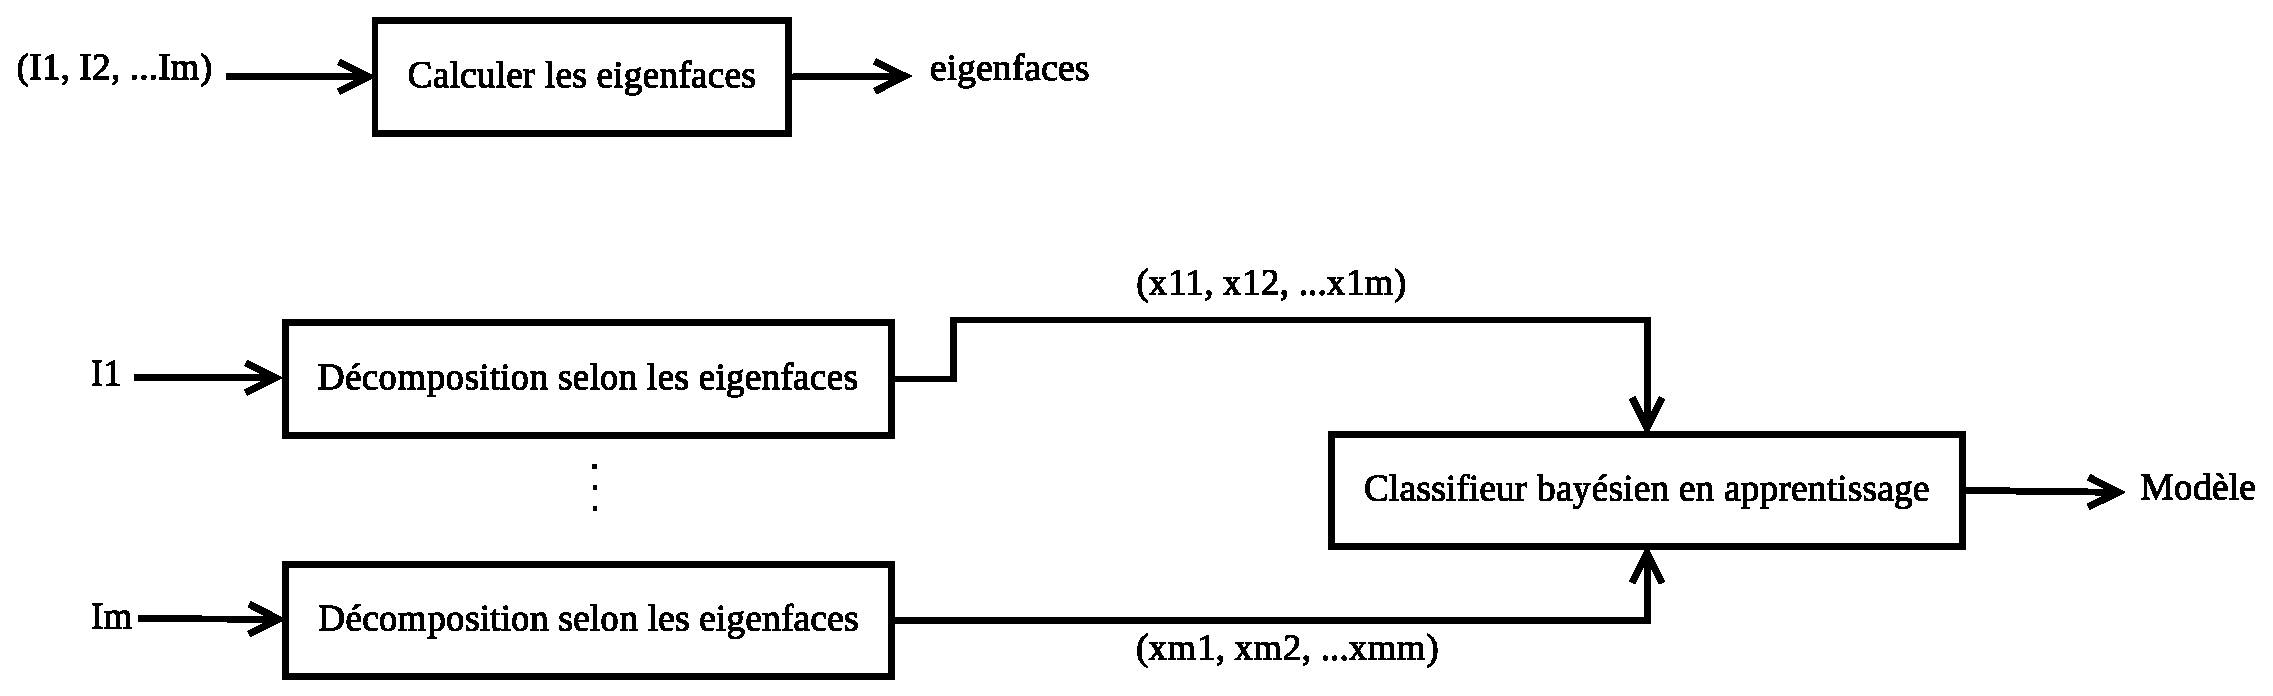
\includegraphics[scale=0.4]{images/article_etapes_apprentissage}
    \caption{Étape d'apprentissage.}
    \label{fig:article:etapes_apprentissage}
\end{figure}
À la fin de cette étape, on aura l'ensemble des eigenfaces et un classifieur 
bayésien entraîné.

\subsubsection{Déploiement du modèle}
Une fois le modèle appris, on peut reconnaître de nouvelles images. Quand on a une nouvelle
image d'un visage, on calcule ses coordonnées dans la base des eigenfaces et on fait
passer ces coordonnées à l'entrée du classifieur bayésien qui nous donne en sortie la
personne à laquelle appartient le visage. Le visage doit appartenir à une personne qui existe
dans la base de données d'entraînement. La figure \ref{fig:article:etapes_deploiement}
résume cette étape.
\begin{figure}[H]
    \centering
    \includegraphics[scale=0.4]{images/article_etapes_deploiement}
    \caption{Système déployé.}
    \label{fig:article:etapes_deploiement}
\end{figure}


\subsection{Résultats obtenus par la méthode}
Les auteurs de \cite{article} ont travaillé sur une base de données
de 200 images de 20 personnes, avec donc 10 images par personne.
Le taux d'images correctement classées est de $70\%$. En normalisant
(centrer, réduire) les valeurs des vecteurs propres (eigenfaces),
les auteurs affirment avoir obtenu un taux de réussite de $89.5\%$.


\subsection{Critique de la méthode de test}
Pour les calculs des eigenfaces, les auteurs de \cite{article} ont
utilisé toutes les images de la base de données (pas de séparation
en données d'entraînement et de test). Ensuite, ils ont fait de la
validation croisée pour entraîner le classifieur bayésien et estimer
le taux de succès de la méthode. Mais étant donné que même les 
données de test ont été utilisées pour la génération des eigenfaces,
les résultats obtenus sont biaisés, les données de tests ne doivent
pas du tout entrer dans le processus de génération du modèle.
    
    \chapter{Notre implémentation}
    \subsection{Base de données}
La base de données d'images que nous avons utilisé est la base AT\&T\\
(lien : \url{http://www.cl.cam.ac.uk/research/dtg/attarchive/facedatabase.html}).
C'est une base de 400 images de visages de 40 personnes, avec 10 images 
par personne. Les visages sont bien centrés sur l'image et l'arrière-plan
est très peu apparent ; ça correspond au genre d'images obtenues après une étape de 
détection (localisation) de visage. La figure \ref{fig:implementation:bdd_exemple} montre
un échantillon des images de la base.
\begin{figure}[H]
    \centering
    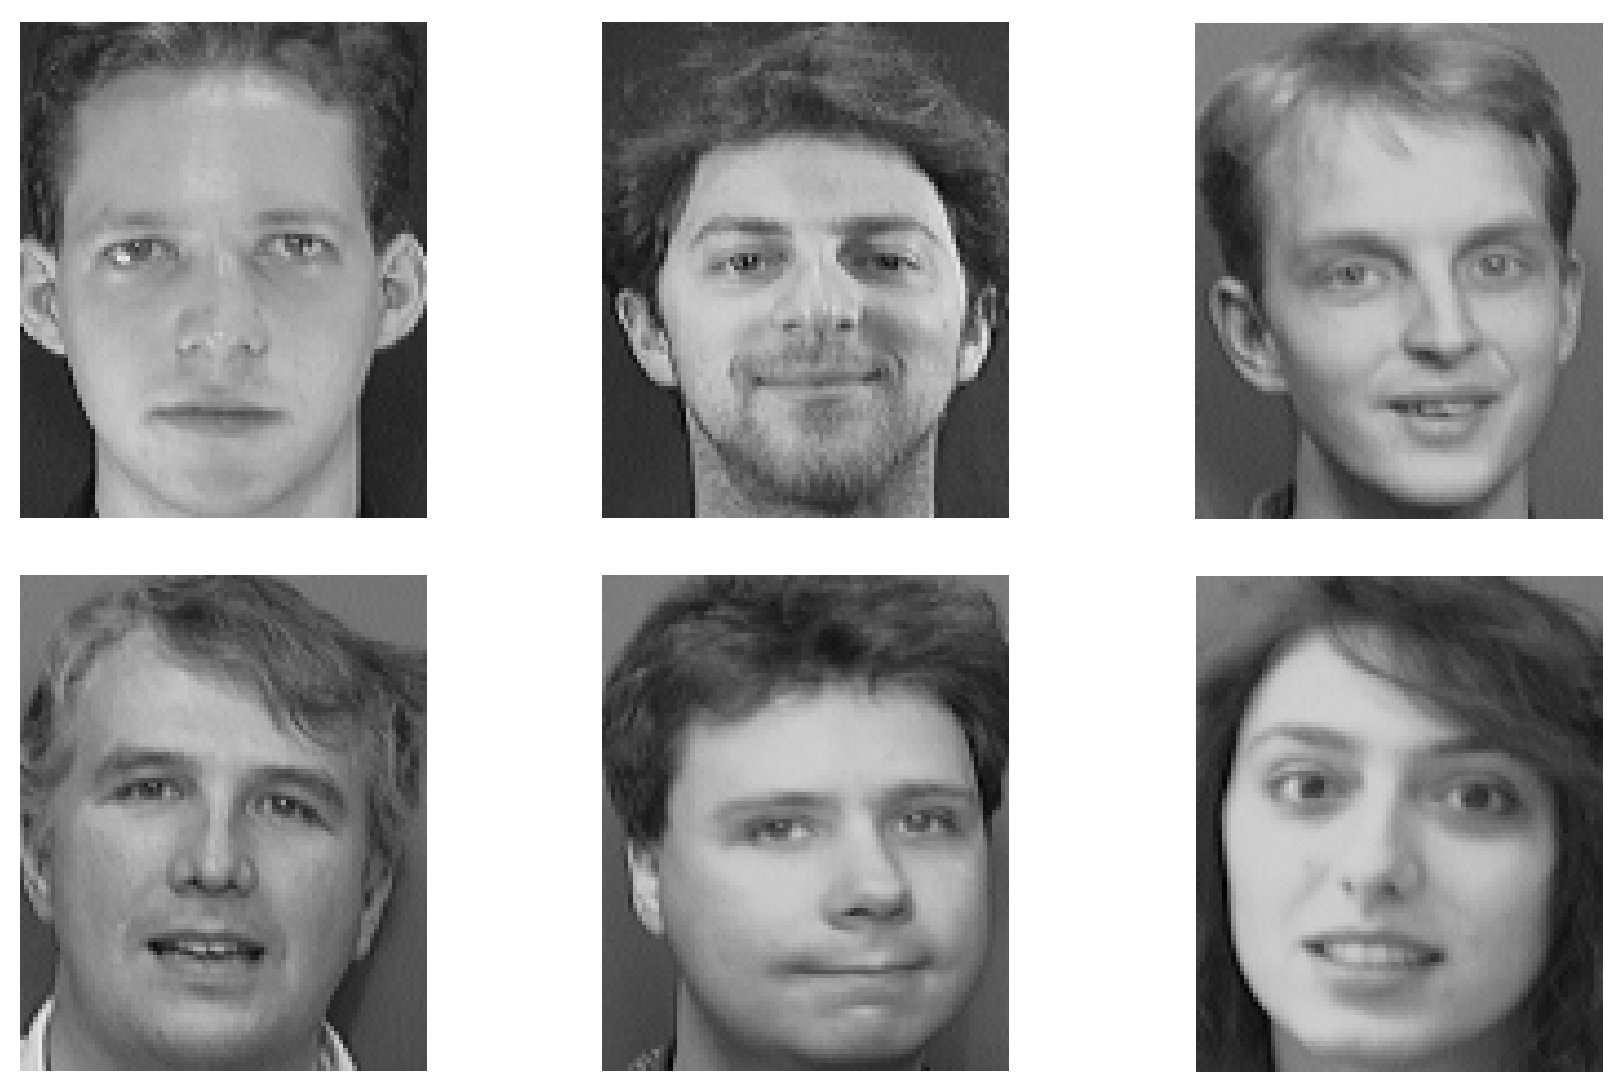
\includegraphics[scale=0.4]{images/bdd_exemple}
    \caption{Échantillon des images de la base de données AT\&T.}
    \label{fig:implementation:bdd_exemple}
\end{figure}
Les images sont en niveaux de gris et ont une taille de $92 \times 112$.


\subsection{Méthodologie de test}
Étant donné que nous avons un nombre limité d'images, nous ne pouvons pas
nous permettre de partitionner l'ensemble des 400 images en données 
d’entraînement et de test ; la variance des résultats obtenus les rendrait
inexploitable (à vrai dire on a essayé ça, le taux de classification correcte
varie entre $50\%$ et $80\%$ pour deux choix aléatoires des données d'entraînement
et de test, ce qui est une marge trop large).

Pour tester les performances du système, nous allons utiliser la validation croisée.
La validation croisée est une méthode d’estimation des performances d'un algorithme
d'apprentissage automatique. On divise l'ensemble des images en $k$ échantillons, 
puis on sélectionne un des $k$ échantillons comme ensemble de test et les $k-1$ autres
échantillons comme ensemble d'apprentissage. On apprend le modèle sur
l'ensemble d'apprentissage et on mesure le taux de classification correcte sur l'ensemble
de test. On répète l'opération en sélectionnant un autre échantillon de test parmi les $k-1$
échantillons qui n'ont pas encore été utilisés pour tester le modèle. 
L'opération se répète ainsi $k$ fois pour de sorte que chaque sous-échantillon ait été utilisé exactement
une fois comme ensemble de test. La moyenne des $k$ taux de classification correcte servira
d'estimation finale du taux de classification correcte du système.

Dans notre cas, nous avons pris $k = 10$. Pour chaque personne,
9 images d'entraînement et une de test pour chaque itération.
À noter que contrairement à ce qui a été fait dans \cite{article},
les eigenfaces ont été calculées en utilisant uniquement les données
d'entraînement, ce qui permet d'avoir une estimation plus correcte 
des performances du système.


\subsection{Résultats obtenus}
Nous avons obtenu un taux de reconnaissance correcte de $68\%$, ce qui est proche
du taux obtenu par \cite{article} sans normalisation des eigenfaces (à savoir $70\%$).
Notre taux de $68\%$ a été obtenu en normalisant les eigenfaces, cette normalisation
n'influence que très peu le taux de reconnaissance.

Il est à mentionner que nous avons travaillé avec 40 classes, et \cite{article}
ont travaillé avec 20 classes. Quand nous réduisons le nombre de classes à 20
(et donc le nombre d'images à 200), nous obtenons un taux de reconnaissance
correcte de $82\%$, ce qui est assez proche du taux de $89.5\%$ obtenu par \cite{article}.
    
    \chapter{Étude de la robustesse du système}
    Nous allons étudier la robustesse du système par rapport au nombre de personne,
le bruit, l'inversion du contraste, la rotation et la translation.


\subsection{Robustesse au nombre de personnes}
Nous avons déjà dit lorsque nous avons présenté nos résultats que quand il y a
40 personnes, le taux de reconnaissances correctes est de $68\%$, alors que quand
il y a 20 personnes, celui-ci est de $82\%$. Ce large écart nous pousse à étudier
l'influence que peut avoir le nombre de personnes sur les performances du système.

La figure \ref{fig:robustness:nombre_de_personnes} montre l'évolution du taux
de reconnaissances correctes en fonction du nombre de personnes. On voit que...

\begin{figure}[H]
    \centering
    \includegraphics[scale=0.5]{images/robustesse_nombre_de_personnes}
\end{figure}
Malheureusement, comme il y a 40 personnes dans la base de données AT\&T, on ne 
peut pas tester pour des valeurs supérieures à 40.


\subsection{Robustesse au bruit}
\subsubsection{Bruit blanc gaussien}
On entraîne le système sur des données non bruitées puis on le teste sur des images
bruitées. La figure \ref{fig:robustness:gaussien:test} montre les variations du taux
de reconnaissances correctes en fonction de la variance $\sigma^2$ du bruit blanc
gaussien.
\begin{figure}[H]
    \centering
    \includegraphics[scale=0.5]{images/robustesse_gaussien_test}
    \caption{Taux de reconnaissance en fonction de la variance du bruit blanc gaussien
    (apprentissage sur des images non bruitées).}
    \label{fig:robustness:gaussien:test}
\end{figure}
Pour mieux visualiser la chose, la figure \ref{fig:robustness:gaussien:exemple} montre
une image non bruitée et la même image avec des bruits gaussiens de différentes variances.
\begin{figure}[H]
    \centering
    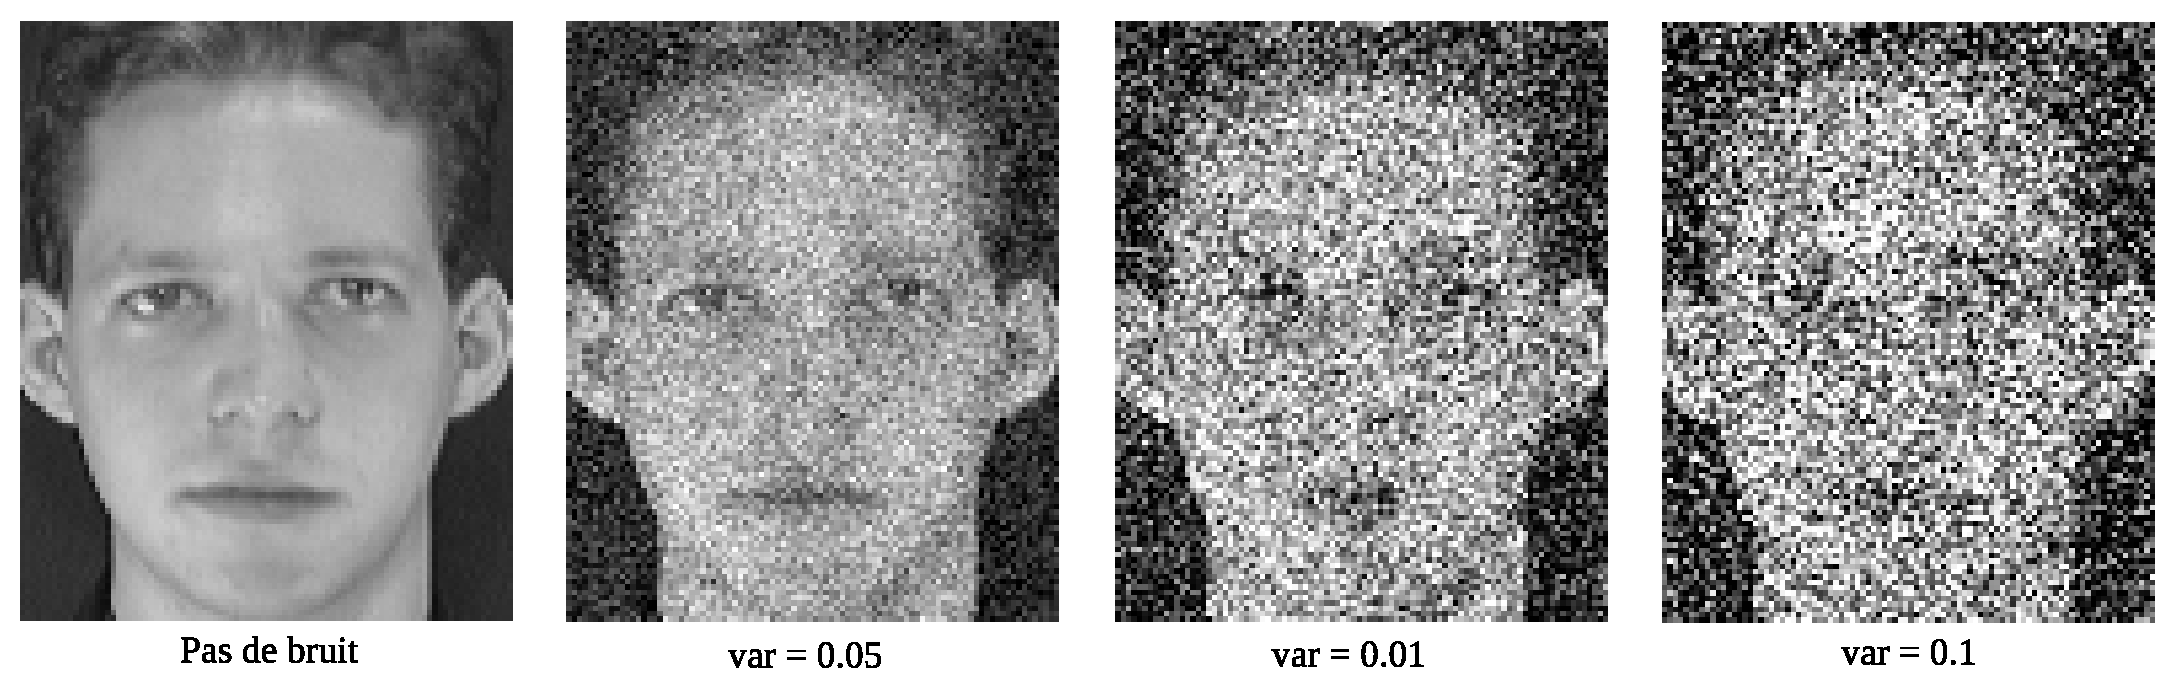
\includegraphics[scale=0.45]{images/robustness_gaussien_exemple}
    \caption{Exemple de bruits blancs gaussiens de différentes variances.}
    \label{fig:robustness:gaussien:exemple}
\end{figure}
Nous voyons que les performances commencent à décroître dès que le bruit
devient apparent. Pour une variance supérieure à $0.1$, on n'attend pas du système
qu'il ait de bonnes performances car même un être humain aurait des difficultés à
reconnaître la personne.

Maintenant, au lieu d'entraîner sur des données non bruitées et de tester sur des 
données bruitées, nous allons introduire un pourcentage ($30\%$) d'images bruitées
dans les images d'entraînement et de test. Le graphe de la figure \ref{fig:robustness:gaussien:tout} 
montre les taux de reconnaissance obtenus pour différentes variances.
\begin{figure}[H]
    \centering
    \includegraphics[scale=0.5]{images/robustesse_gaussien_tout}
    \caption{Taux de reconnaissance en fonction de la variance du bruit blanc gaussien
    (apprentissage sur des images bruitées).}
    \label{fig:robustness:gaussien:touxt}
\end{figure}
Les performances cette fois-ci sont inférieures à celles que nous avions obtenu lorsque nous
avons utilisé uniquement des données non bruitées pour l'entraînement. Nous suspectons que 
l'introduction de bruits dans les données d'entraînement a conduit à une mauvaise reconnaissance
des images non bruitées (en plus des images bruitées).

On conclue que le système est peu robuste aux bruits gaussiens. 
Ces résultats sont toutefois à prendre avec
précaution étant donné le nombre limité d'images disponibles.

\subsubsection{Bruit de Poisson}
La figure \ref{fig:robustness:poisson} montre une image avant et après application d'un bruit de Poisson.
Après avoir entraîné le système sur des images non bruitées, quand on teste sur des images
bruitées (bruit de Poisson), le taux de reconnaissances correctes est de $68\%$, le même que
sur des données non bruitées. On en conclue que le système est robuste aux bruits de Poisson.
\begin{figure}[H]
    \centering
    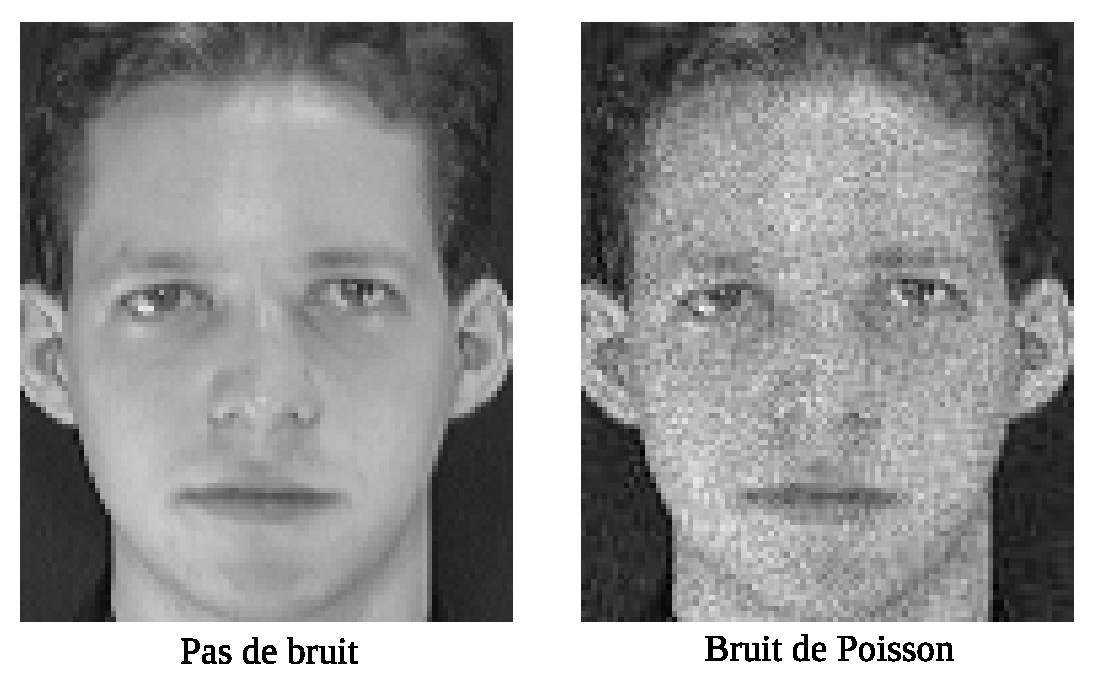
\includegraphics[scale=0.6]{images/exemple_poisson}
    \caption{Exemple d'un bruit de Poisson.}
    \label{fig:robustness:poisson}
\end{figure}

\subsubsection{Bruit Speckle}
On entraîne le système sur des données non bruitées puis on le teste sur des images
bruitées. La figure \ref{fig:robustness:speckle:test} montre les variations du taux
de reconnaissances correctes en fonction de la variance $\sigma^2$ du bruit speckle.
\begin{figure}[H]
    \centering
    \includegraphics[scale=0.5]{images/robustesse_speckle_test}
    \caption{Taux de reconnaissance en fonction de la variance du bruit speckle.}
    \label{fig:robustness:speckle:test}
\end{figure}
Pour mieux visualiser la chose, la figure \ref{fig:robustness:speckle:exemple} montre
une image non bruitée et la même image avec des bruits speckle de différentes variances.
\begin{figure}[H]
    \centering
    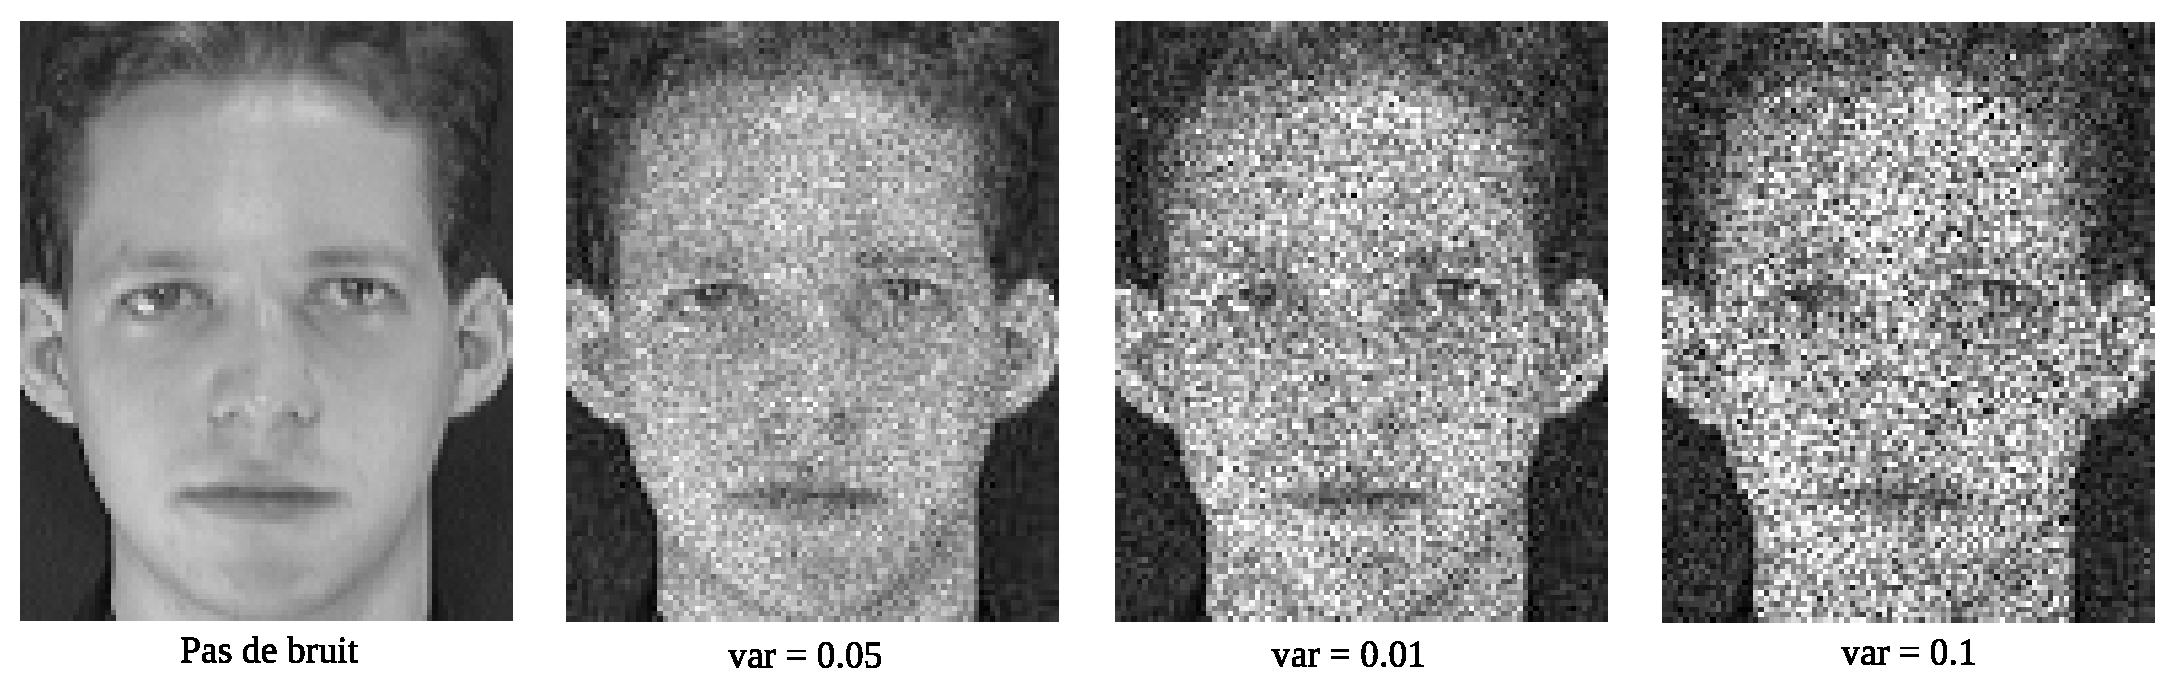
\includegraphics[scale=0.45]{images/robustness_speckle_exemple}
    \caption{Exemple de bruits speckle de différentes variances.}
    \label{fig:robustness:speckle:exemple}
\end{figure}

Nous voyons qu'il y a une détérioration des performances à mesure que le bruit speckle
devient apparent, mais le système conserve quand-même un taux de reconnaissance assez 
satisfaisant (comparé à ses performances dans le cas sans bruits). On en conclue que le
système est assez robuste au bruit speckle (Il n'est pas totalement robuste, ses performances
diminuent là où celles d'un être humain resteraient les mêmes).

\subsubsection{Bruit poivre et sel}
On entraîne le système sur des données non bruitées puis on le teste sur des images
bruitées. La figure \ref{fig:robustness:sp:test} montre les variations du taux
de reconnaissances correctes en fonction du pourcentage des pixels de l'image affectés
par le bruit poivre et sel.
\begin{figure}[H]
    \centering
    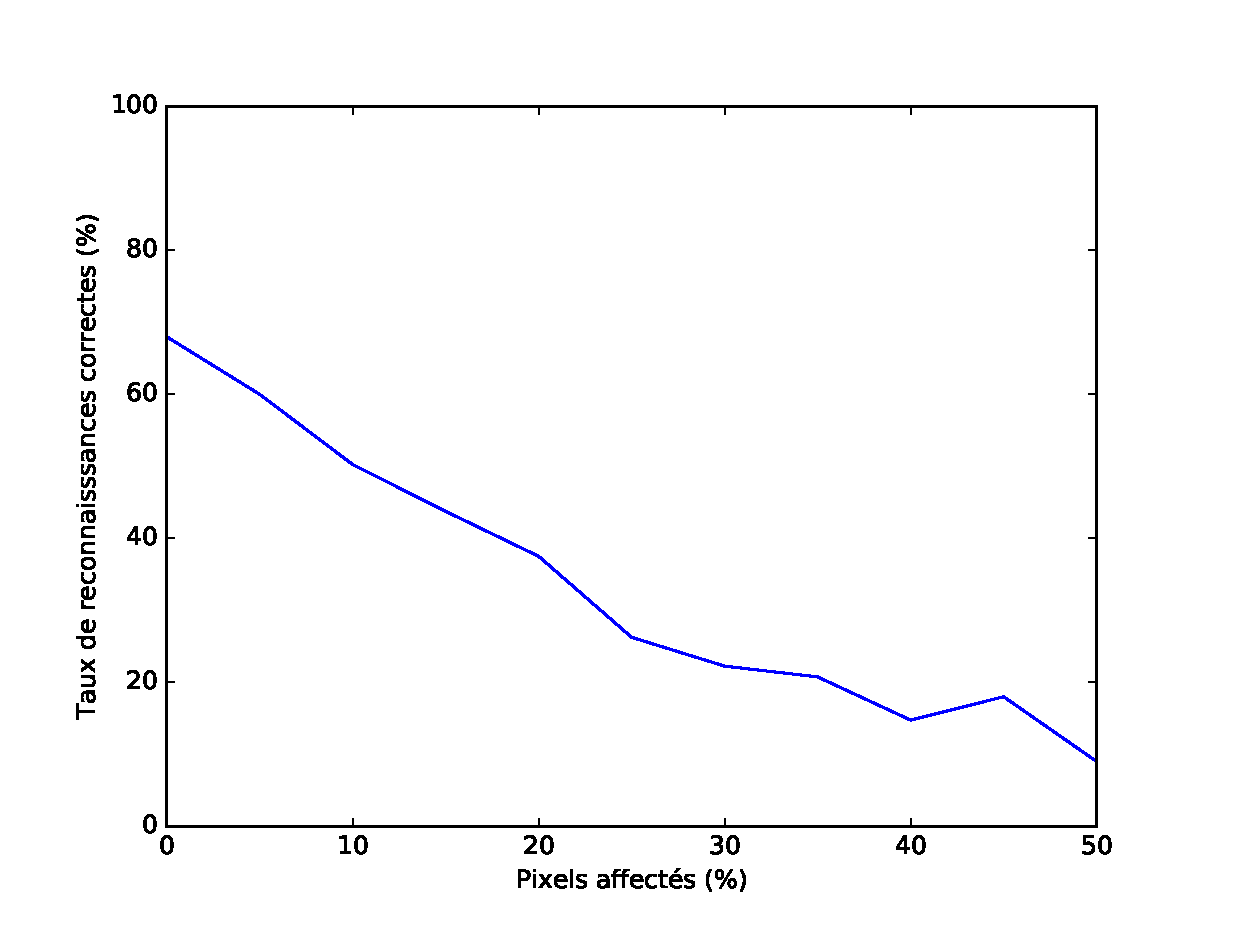
\includegraphics[scale=0.5]{images/robustesse_sp_test}
    \caption{Taux de reconnaissance en fonction du pourcentage des pixels bruités (bruit poivre et sel).}
    \label{fig:robustness:sp:test}
\end{figure}
Pour mieux visualiser la chose, la figure \ref{fig:robustness:sp:exemple} montre
une image non bruitée et la même image avec des bruits poivre et sel affectant 
différents pourcentages de pixels.
\begin{figure}[H]
    \centering
    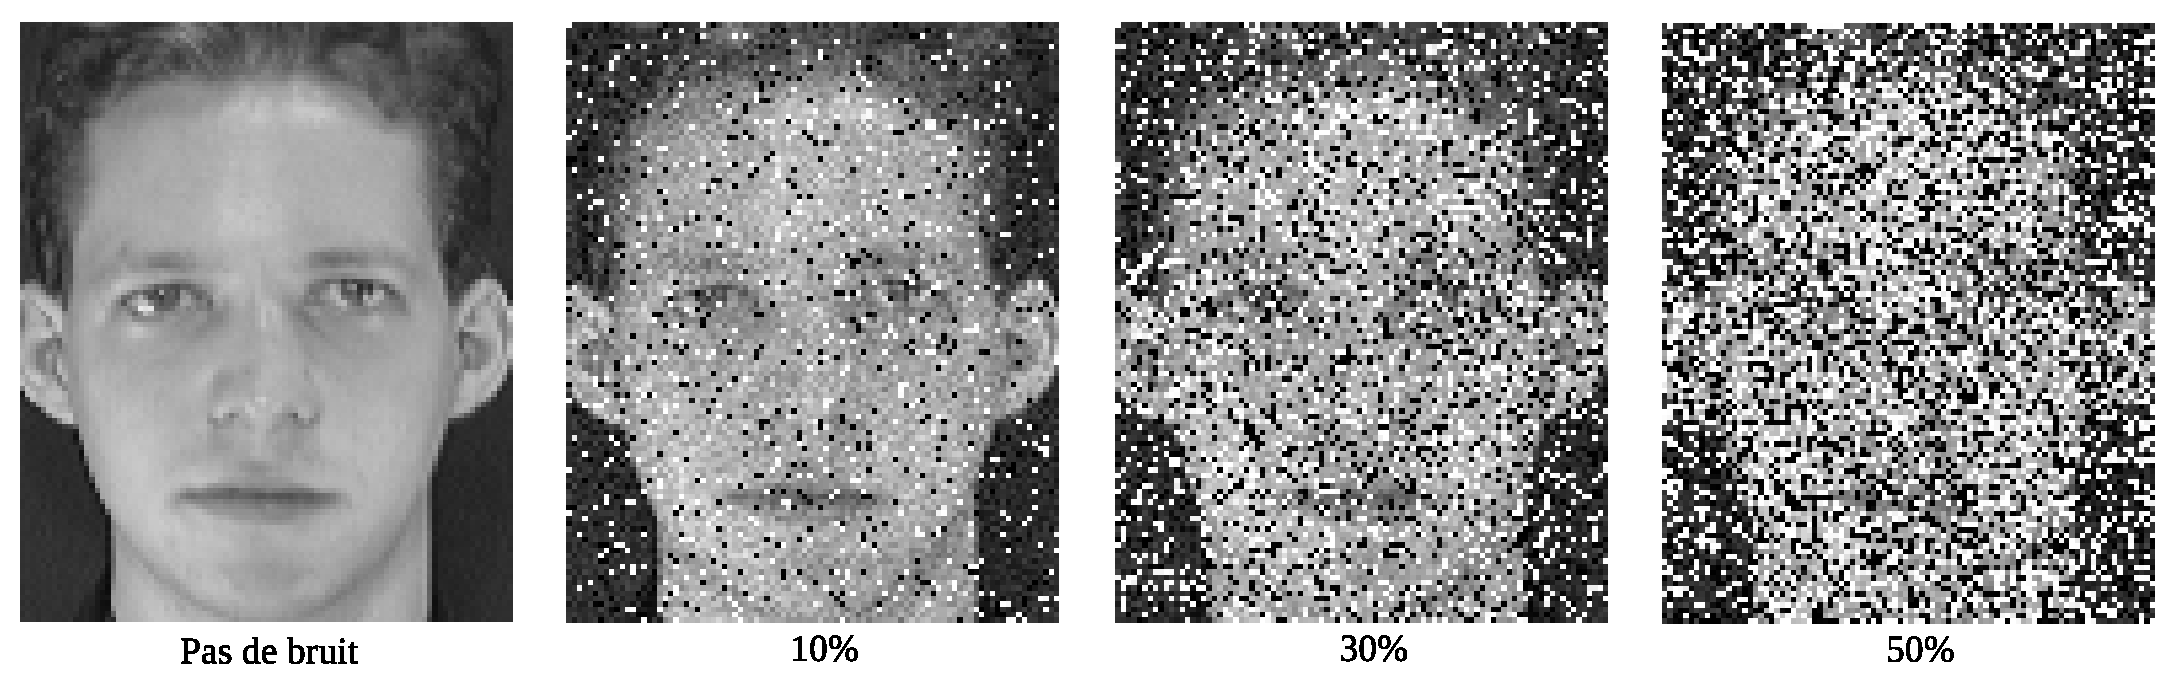
\includegraphics[scale=0.45]{images/robustness_sp_exemple}
    \caption{Exemple de bruits poivre et sel affectant différents pourcentages de pixels
    (apprentissage sur des images non bruitées).}
    \label{fig:robustness:sp:exemple}
\end{figure}

Nous voyons que les performances commencent à décroître dès que le bruit
devient apparent, donc à la base, le système n'est pas robuste aux bruits
poivre et sel.

Maintenant, au lieu d'entraîner sur des images non bruitées et de tester sur des 
images bruitées, nous allons introduire un pourcentage ($30\%$) d'images bruitées
dans les images d'entraînement et de test. Le graphe de la figure \ref{fig:robustness:sp:tout} 
montre les taux de reconnaissance obtenus pour différents pourcentages de pixels affectés.
\begin{figure}[H]
    \centering
    \includegraphics[scale=0.5]{images/robustesse_sp_tout}
    \caption{Taux de reconnaissance en fonction du pourcentage des pixels affectés par le bruit
    poivre et sel (apprentissage sur des images bruitées).}
    \label{fig:robustness:sp:tout}
\end{figure}
Les performances cette fois-ci sont inférieures à celles que nous avions obtenu lorsque nous
avons utilisé uniquement des données non bruitées pour l'entraînement. Nous suspectons que 
l'introduction de bruits dans les images d'entraînement a conduit à une mauvaise reconnaissance
des images non bruitées (en plus des images bruitées).

On conclue que le système n'est pas robuste aux bruits poivre et sel.


\subsection{Robustesse à l'inversion de contraste}
Quand nous entraînons le système sur des images dont le contraste n'a pas été inversé et nous
ne testons que sur des images dont le contraste a été inversé, le taux de reconnaissances
correctes est de $0\%$! Vraiment pas robuste donc.

Quand nous inversons le contraste de $30\%$ des images d'entraînement et de test, le taux de
reconnaissances correctes obtenu est de $35\%$.

Conclusion : le système n'est pas robuste à l'inversion de contraste (contrairement à l'etre
humain qui en général peut reconnaître sans problème une personne dont le contraste de l'image
du visage a été inversé).
    
    \chapter*{Conclusion}
    \addcontentsline{toc}{chapter}{Conclusion}
    Dans ce projet, nous avons vu une méthode de reconnaissance faciale
basée sur les eigenfaces et utilisant un classifieur bayésien. La 
méthode se distingue des approches actuelles par le faite qu'elle soit
très rapide à implémenter (le modèle est généré rapidement).

Coté taux de reconnaissance, on arrive à un taux de près de $70\%$, ce qui
est bien loin des performances des systèmes actuels basés sur l'apprentissage
profond.

Ce système de reconnaissance est assez robuste aux bruits speckle et de poisson,
il l'est beaucoup moins aux bruits gaussiens et poivre et sel. Il n'est également
pas du tout robuste à l'inversion de contraste et est très peu robuste à la translation.
Pour avoir une assez bonne robustesse à la rotation, il faut introduire des images
retournées lors de la construction du modèle (dans les images d’entraînement).
    
    \newpage
    \bibliographystyle{alpha}
    \bibliography{references}
    
\end{document}